\subsection{Loading File Module}
\label{sec:LoadingFileModule}
Loading File Module offers users to choose a crisp database and its schema from local file system.
It parses database schema and generates  a table called Attribute to store information (name of attribute, type of attribute, range of attribute), on which fuzzy concepts are built.

\subsubsection{Database and its schema}
Crisp database is in a prolog file with extension ``.pl", and its schema is in a XML file with extension ``.xml". Crisp database is simply one predicate prolog program, the predicate is the name of table, and its arguments are terms of atom. Each atom is considered as an entry in the table. The schema of database is presented in .xml file, which stores table name, primary key and attributes information.
There are examples of crisp database in .pl file and its schema in .xml file.

%Explain db file
\begin{ex}
In .pl file, house is the only predicate, and it is the name of table. All the atoms in .pl file are entries of the table house.
\lstinputlisting{house.pl}
\end{ex}

%Explain db Schema file
\begin{ex}
As shown in .xml file, the name of table is house, the primary key is house\_code. The attributes of table house are type, size, number of rooms, price, distance from center, close to beach. The information about domain of each attribute is also included.
\lstinputlisting{house.xml}
\end{ex}

\subsubsection{How to use interface of Loading File Module}
The web interface of Loading File Module is shown in figure \ref{fig:LFI}. Three steps  to load a database.
\begin{enumerate}
\item Choose crisp database from Db selection box
\item Choose corresponding database schema from Xml selection box
\item Click Button Load
\end{enumerate}
In the last step, system stores file information in model ``InputFile" and parses .xml file into two models, one is ``Table", the other is ``Attribute". All the models are in file models.py.
\begin{figure}[htb]
\begin{center}
\leavevmode
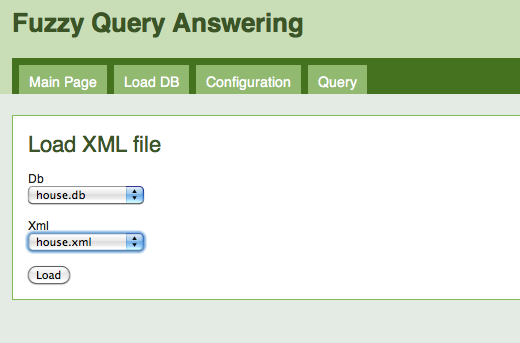
\includegraphics[scale=0.7]{LoadFile.png}
\end{center}
\caption{Loading File Interface}
\label{fig:LFI}
\end{figure}




